\documentclass[11pt, a4paper]{article}
\usepackage{amsmath, amssymb, titling}
\usepackage[margin=2cm]{geometry}
\usepackage[colorlinks=true, linkcolor=black, urlcolor=black, citecolor=black]{hyperref}
\usepackage{graphicx}
\usepackage{caption}
\usepackage{subcaption}
\usepackage{float}

\renewcommand\maketitlehooka{\null\mbox{}\vfill}
\renewcommand\maketitlehookd{\vfill\null}

\title{Computational Fluid Dynamics}
\author{Almog Dobrescu\\\\ID 214254252}

\begin{document}

\maketitle

\thispagestyle{empty}
\newpage
\setcounter{page}{1}

\tableofcontents
\vfil
\listoffigures
\newpage

\section{Mathematical Problem}
The Burgers Equation:
\begin{equation}
    \frac{\partial u}{\partial t} + u\frac{\partial u}{\partial y} = \frac{\partial}{\partial y}\left(\mu\frac{\partial u}{\partial y}\right)
\end{equation}
By neglection the convective term, the parabolic model equation is obtained:
\begin{align}
    \frac{\partial u}{\partial t} &= \frac{\partial}{\partial y}\left(\mu\frac{\partial u}{\partial y}\right)\\
    \frac{\partial u}{\partial t} &= \mu\frac{\partial^2 u}{\partial y^2}\\
    \mu &= 1.0
\end{align}
Boundary and initial conditions:
\begin{equation}
    u_{(y_0, t)} = u_0 \hspace{1cm} u_{(y_1, t)} = u_1 \hspace{1cm} u_{(y, t=0)} = f_{(y)}
\end{equation}

\section{Numerical Scheme}
A general explicit-implicit scheme for constant $\mu$ is given by:
\begin{equation}
    u^{n+1}_i = u^n_i + \frac{\mu\Delta t}{\Delta y^2}\delta_{yy}\left[\left(1-\alpha\right)u^n_i+\alpha u^{n+1}_i\right]
\end{equation}
where:
\begin{equation}
    \alpha = \left\{\begin{matrix}
        0 & \text{Explicit}\\
        \frac{1}{2} & \text{Crank-Nicolson}\\
        1 & \text{Implicit}
    \end{matrix}\right.
\end{equation}
and the order is:
\begin{equation}
    \left[\Delta x^2, \Delta\left(\frac{1}{2}-\alpha\right)\right]
\end{equation}
In delta form:
\begin{equation}
    \left(I-\alpha\frac{\mu\Delta t}{\Delta y^2}\delta_{yy}\right)\Delta u^n_i = \frac{\mu\Delta t}{\Delta y^2}\delta_{yy}u^n_i
\end{equation}
Applying the operators:
\begin{align}
    \Delta u^n_i - \alpha\frac{\mu\Delta t}{\Delta y^2}\delta_{yy}\left(\Delta u^n_i\right) &= \frac{\mu\Delta t}{\Delta y^2}\delta_{yy}\left(u^n_i\right)\\
    \Delta u^n_i - \alpha\frac{\mu\Delta t}{\Delta y^2}\delta_{y}\left(\Delta u^n_{\left(y_i+\frac{\Delta y}{2}\right)} - \Delta u^n_{\left(y_i-\frac{\Delta y}{2}\right)}\right) &= \frac{\mu\Delta t}{\Delta y^2}\delta_{y}\left(u^n_{\left(y_i+\frac{\Delta y}{2}\right)} - u^n_{\left(y_i-\frac{\Delta y}{2}\right)}\right)\\
    \Delta u^n_i - \alpha\frac{\mu\Delta t}{\Delta y^2}\left(\scriptstyle\Delta u^n_{\left(y_i+\Delta y\right)} - 2\Delta u^n_{\left(y_i\right)} + \Delta u^n_{\left(y_i - \Delta y\right)}\right) &= \frac{\mu\Delta t}{\Delta y^2}\left(\scriptstyle u^n_{\left(y_i+\Delta y\right)} - 2u^n_{\left(y_i\right)} + u^n_{\left(y_i-\Delta y\right)}\right)\\
    \Delta u^n_i - \alpha\frac{\mu\Delta t}{\Delta y^2}\left(\Delta u^n_{i+1}-2\Delta u^n_i + \Delta u^n_{i-1}\right) &= \frac{\mu\Delta t}{\Delta y^2}\left(u^n_{i+1} - 2u^n_{i} + u^n_{i-1}\right)\\
    A_i\Delta u^n_{i-1}+B_i\Delta u^n_i+C_i\Delta u^n_{i+1} &= D_i
\end{align}
where:
\begin{align}
    A'_i &= - \alpha\frac{\mu\Delta t}{\Delta y^2}\\
    B'_i &= 1 + 2 \alpha\frac{\mu\Delta t}{\Delta y^2}\\
    C'_i &= - \alpha\frac{\mu\Delta t}{\Delta y^2}\\
    D'_i &= \frac{\mu\Delta t}{\Delta y^2}\left(u^n_{i+1} - 2u^n_{i} + u^n_{i-1}\right)
\end{align}
and advancing the solution with:
\begin{equation}
    u^{n+1}_i = u^n_i + \Delta u^n_i
\end{equation}
To reduce problems of big flouting point numbers, define \emph{r}:
\begin{equation}
    r \triangleq \frac{\mu\Delta t}{\Delta y^2}
\end{equation}
After dividing by \emph{r}:
\begin{align}
    A_i &= - \alpha\\
    B_i &= \frac{1}{r} + 2 \alpha\\
    C_i &= - \alpha\\
    D_i &= \left(u^n_{i+1} - 2u^n_{i} + u^n_{i-1}\right)
\end{align}
\subsection{For $\alpha = 0$}
When $\alpha = 0$ The shceme simplifies to:
\begin{equation}
    \Delta u^n_i = rD_i
\end{equation}

\subsection{For $\alpha \neq 0$}
When $\alpha \neq 0$ in order to calculate $\Delta u^n_i$ it is needed to invert matrix as follows:
\begin{equation}
    \begin{pmatrix}
        B_1 & C_1 & 0 & \cdots & \cdots & \cdots & 0 \\
        A_2 & B_2 & C_2 & 0 & \cdots & \cdots & 0 \\
        0 & \ddots & \ddots & \ddots & 0 & \cdots & 0 \\
        0 & 0 & A_i & B_i & C_i & 0 & 0 \\
        0 & \cdots & 0 & \ddots & \ddots & \ddots & 0 \\
        0 & \cdots & \cdots & 0 & A_{N-2} & B_{N-2} & C_{N-2} \\
        0 & 0 & \cdots & \cdots & 0 & A_{N-1} &B_{N-1}
    \end{pmatrix}
    \begin{pmatrix}
        \Delta u_1\\
        \Delta u_2\\
        \cdots\\
        \cdots\\
        \cdots\\
        \Delta u_{N-2}\\
        \Delta u_{N-1}
    \end{pmatrix}
    =
    \begin{pmatrix}
        D_1-A_1\cdot u_0\\
        D_2\\
        \cdots\\
        \cdots\\
        \cdots\\
        D_{N-2}\\
        D_{N-1}-C_{N-1}\cdot u_N
    \end{pmatrix}
\end{equation}
\subsection{In Our Case}
\begin{equation}
    y_0 = 0 \hspace{1cm}
    u_0 = 0 \hspace{1cm}
    y_1 = 1 \hspace{1cm}
    u_1 = 1 \hspace{1cm}
    f_{(y)} = 1 \hspace{1cm}
    N = 11
\end{equation}
The scheme considered converged when the size of the RHS drops by 6 order of magnitude.
\newpage

\section{Stability Analysis}
According to the "von Neumann Stability Analysis", the error between the differential and numerical equation is given by:
\begin{equation}
    \varepsilon = N-D
\end{equation}
where:
\begin{equation}
    \varepsilon(y,t)=\sum_{m}c_m(t)e^{ik_my}
\end{equation}
since the analysis is linear, one can choose one element from the series. Morover, the error becomes:
\begin{equation}
    \varepsilon^n=Z^ne^{iky}
\end{equation}
The constant"\emph{k}" is the wave number theat is related to the initial error.
\begin{equation}
    Z=e^{\lambda\Delta t} \Rightarrow Z^n = e^{\lambda n\Delta t} = e^{\lambda t}
\end{equation}
Any element of the error therefore takes the form:
\begin{equation}
    \varepsilon^n = e^{\lambda  t}e^{iky}
\end{equation}
The ratio between consecutive errors is the \emph{amplification factor}, names "\emph{G}":
\begin{equation}
    G \triangleq \frac{\varepsilon^{n+1}}{\varepsilon^n} = e^{\lambda\Delta t}
\end{equation}
The condition for Stability:
\begin{equation}
    |G| < 1
\end{equation}
The error must satisfies the finite difference equation:
\begin{equation}
    \Delta \varepsilon^n_i - \alpha\frac{\mu\Delta t}{\Delta y^2}\left(\Delta \varepsilon^n_{i+1}-2\Delta \varepsilon^n_i + \Delta \varepsilon^n_{i-1}\right) = \frac{\mu\Delta t}{\Delta y^2}\left(\varepsilon^n_{i+1} - 2\varepsilon^n_{i} + \varepsilon^n_{i-1}\right)
\end{equation}
Where:
\begin{align}
    \Delta\varepsilon^n_i = \varepsilon^{n+1}_i - \varepsilon^n_i &=e^{\lambda\left(t+\Delta t\right)}e^{iky} - e^{\lambda t}e^{iky} = e^{\lambda t}e^{iky}\left(e^{\lambda\Delta t}-1\right)\\
    \Delta\varepsilon^n_{i+1} = \varepsilon^{n+1}_{i+1} - \varepsilon^n_{i+1} &= e^{\lambda\left(t+\Delta t\right)}e^{ik\left(y+\Delta y\right)} - e^{\lambda t}e^{ik\left(y+\Delta y\right)} = e^{\lambda t}e^{ik\left(y+\Delta y\right)}\left(e^{\lambda\Delta t}-1\right)\\
    \Delta\varepsilon^n_{i-1} = \varepsilon^{n+1}_{i-1} - \varepsilon^n_{i-1} &= e^{\lambda\left(t+\Delta t\right)}e^{ik\left(y-\Delta y\right)} - e^{\lambda t}e^{ik\left(y-\Delta y\right)} = e^{\lambda t}e^{ik\left(y-\Delta y\right)}\left(e^{\lambda\Delta t}-1\right)
\end{align}
Substitut the values:
\begin{equation}
    \begin{matrix}
        \displaystyle\left(e^{\lambda t}e^{iky} - \alpha\frac{\mu\Delta t}{\Delta y^2}\left(e^{\lambda t}e^{ik\left(y+\Delta y\right)} - 2e^{\lambda t}e^{iky} + e^{\lambda t}e^{ik\left(y-\Delta y\right)}\right)\right)\left(e^{\lambda\Delta t}-1\right) =\\
        \displaystyle= \frac{\mu\Delta t}{\Delta y^2}\left(e^{\lambda t}e^{ik\left(y+\Delta y\right)} - 2e^{\lambda t}e^{iky} + e^{\lambda t}e^{ik\left(y-\Delta y\right)}\right)
    \end{matrix}
\end{equation}
Dividing by $e^{\lambda t}e^{iky}$:
\begin{equation}
    \left(1-\alpha\frac{\mu\Delta t}{\Delta y^2}\left(e^{ik\Delta y} -2 + e^{-ik\Delta y}\right)\right)\left(e^{\lambda t}-1\right) = \frac{\mu\Delta t}{\Delta y^2}\left(e^{ik\Delta y} -2 + e^{-ik\Delta y}\right)
\end{equation}
Define:
\begin{equation}
    \begin{matrix}
        \displaystyle r \triangleq \frac{\mu\Delta t}{\Delta y^2}, &\displaystyle A \triangleq e^{ik\Delta y}-2+e^{ik\Delta y}=2\cos\beta-2, & \displaystyle \beta \triangleq k\Delta y
    \end{matrix}
\end{equation}
\newpage
\noindent After substitution and rearranging we get:
\begin{equation}
    e^{\lambda t}-1 = \frac{rA}{1-\alpha rA}
\end{equation}
$$\Downarrow$$
\begin{equation}
    G = e^{\lambda t} = 1+\frac{rA}{1-\alpha rA}
\end{equation}
For stability:
\begin{equation}
    |G|<1 \Rightarrow \left|1+\frac{rA}{1-\alpha rA}\right| < 1
\end{equation}
% \begin{equation}
%     -1<\frac{1-4r(1-\alpha)}{1+4r\alpha}<1
% \end{equation}
% \begin{align}
%     -1<\frac{1-4r(1-\alpha)}{1+4r\alpha} \hspace{0.5cm}\emph{and}&\hspace{0.5cm} \frac{1-4r(1-\alpha)}{1+4r\alpha}<1\\
%     \frac{1-4r(r-\alpha)+1+4r\alpha}{1+4r\alpha}>0 \hspace{0.5cm}\emph{and}&\hspace{0.5cm} \frac{1-4r(1-\alpha)-1-4r\alpha}{1+4r\alpha}<0\\
%     2-4r^2+8r\alpha = 0 \hspace{0.5cm} 1+4r\alpha\neq 0 \hspace{0.5cm}\emph{and}&\hspace{0.5cm} -4r\alpha = 0 \hspace{0.5cm} 1+4r\alpha \neq 0
% \end{align}
For $\alpha = 0$:
\begin{align*}
        G = 1+rA\\
        \left|1-4r\right| < 1\\
        -1< 1-4r <1\\
        -2< -4r <0\\
        0< 4r <2\\
        0< r <\frac{1}{2}
\end{align*}
\begin{equation}
    \Delta t < \frac{\Delta y^2}{2\mu}
    \label{eq45}
\end{equation}
For $\alpha = 1$:
\begin{equation*}
    G = \frac{1}{1-rA}
\end{equation*}
\begin{equation}
    \begin{matrix}
        \displaystyle\left|\frac{1}{1-rA}\right|<1 & A \leq 0
    \end{matrix}
\end{equation}
$$\Downarrow$$
\begin{center}
    smaller for every \emph{r} ($\Delta t$)
\end{center}
For every $\alpha$ and $\Delta t\rightarrow\infty$:
\begin{equation}
    \lim_{\Delta t\rightarrow\infty}\left|G\right|=\frac{1-\alpha}{\alpha}
\end{equation}
Which means that stability for infinite time step:
\begin{equation}
    \alpha \left\{\begin{matrix}
        \displaystyle<\frac{1}{2} & \text{Unstable} \\\\
        \displaystyle=\frac{1}{2} & \text{Neutrally stable} \\\\
        \displaystyle>\frac{1}{2} & Stable
    \end{matrix}\right.
\end{equation}



\newpage

\section{The Computer Program}
\subsection{Flow Chart}
\begin{figure}[H]
    \centering
    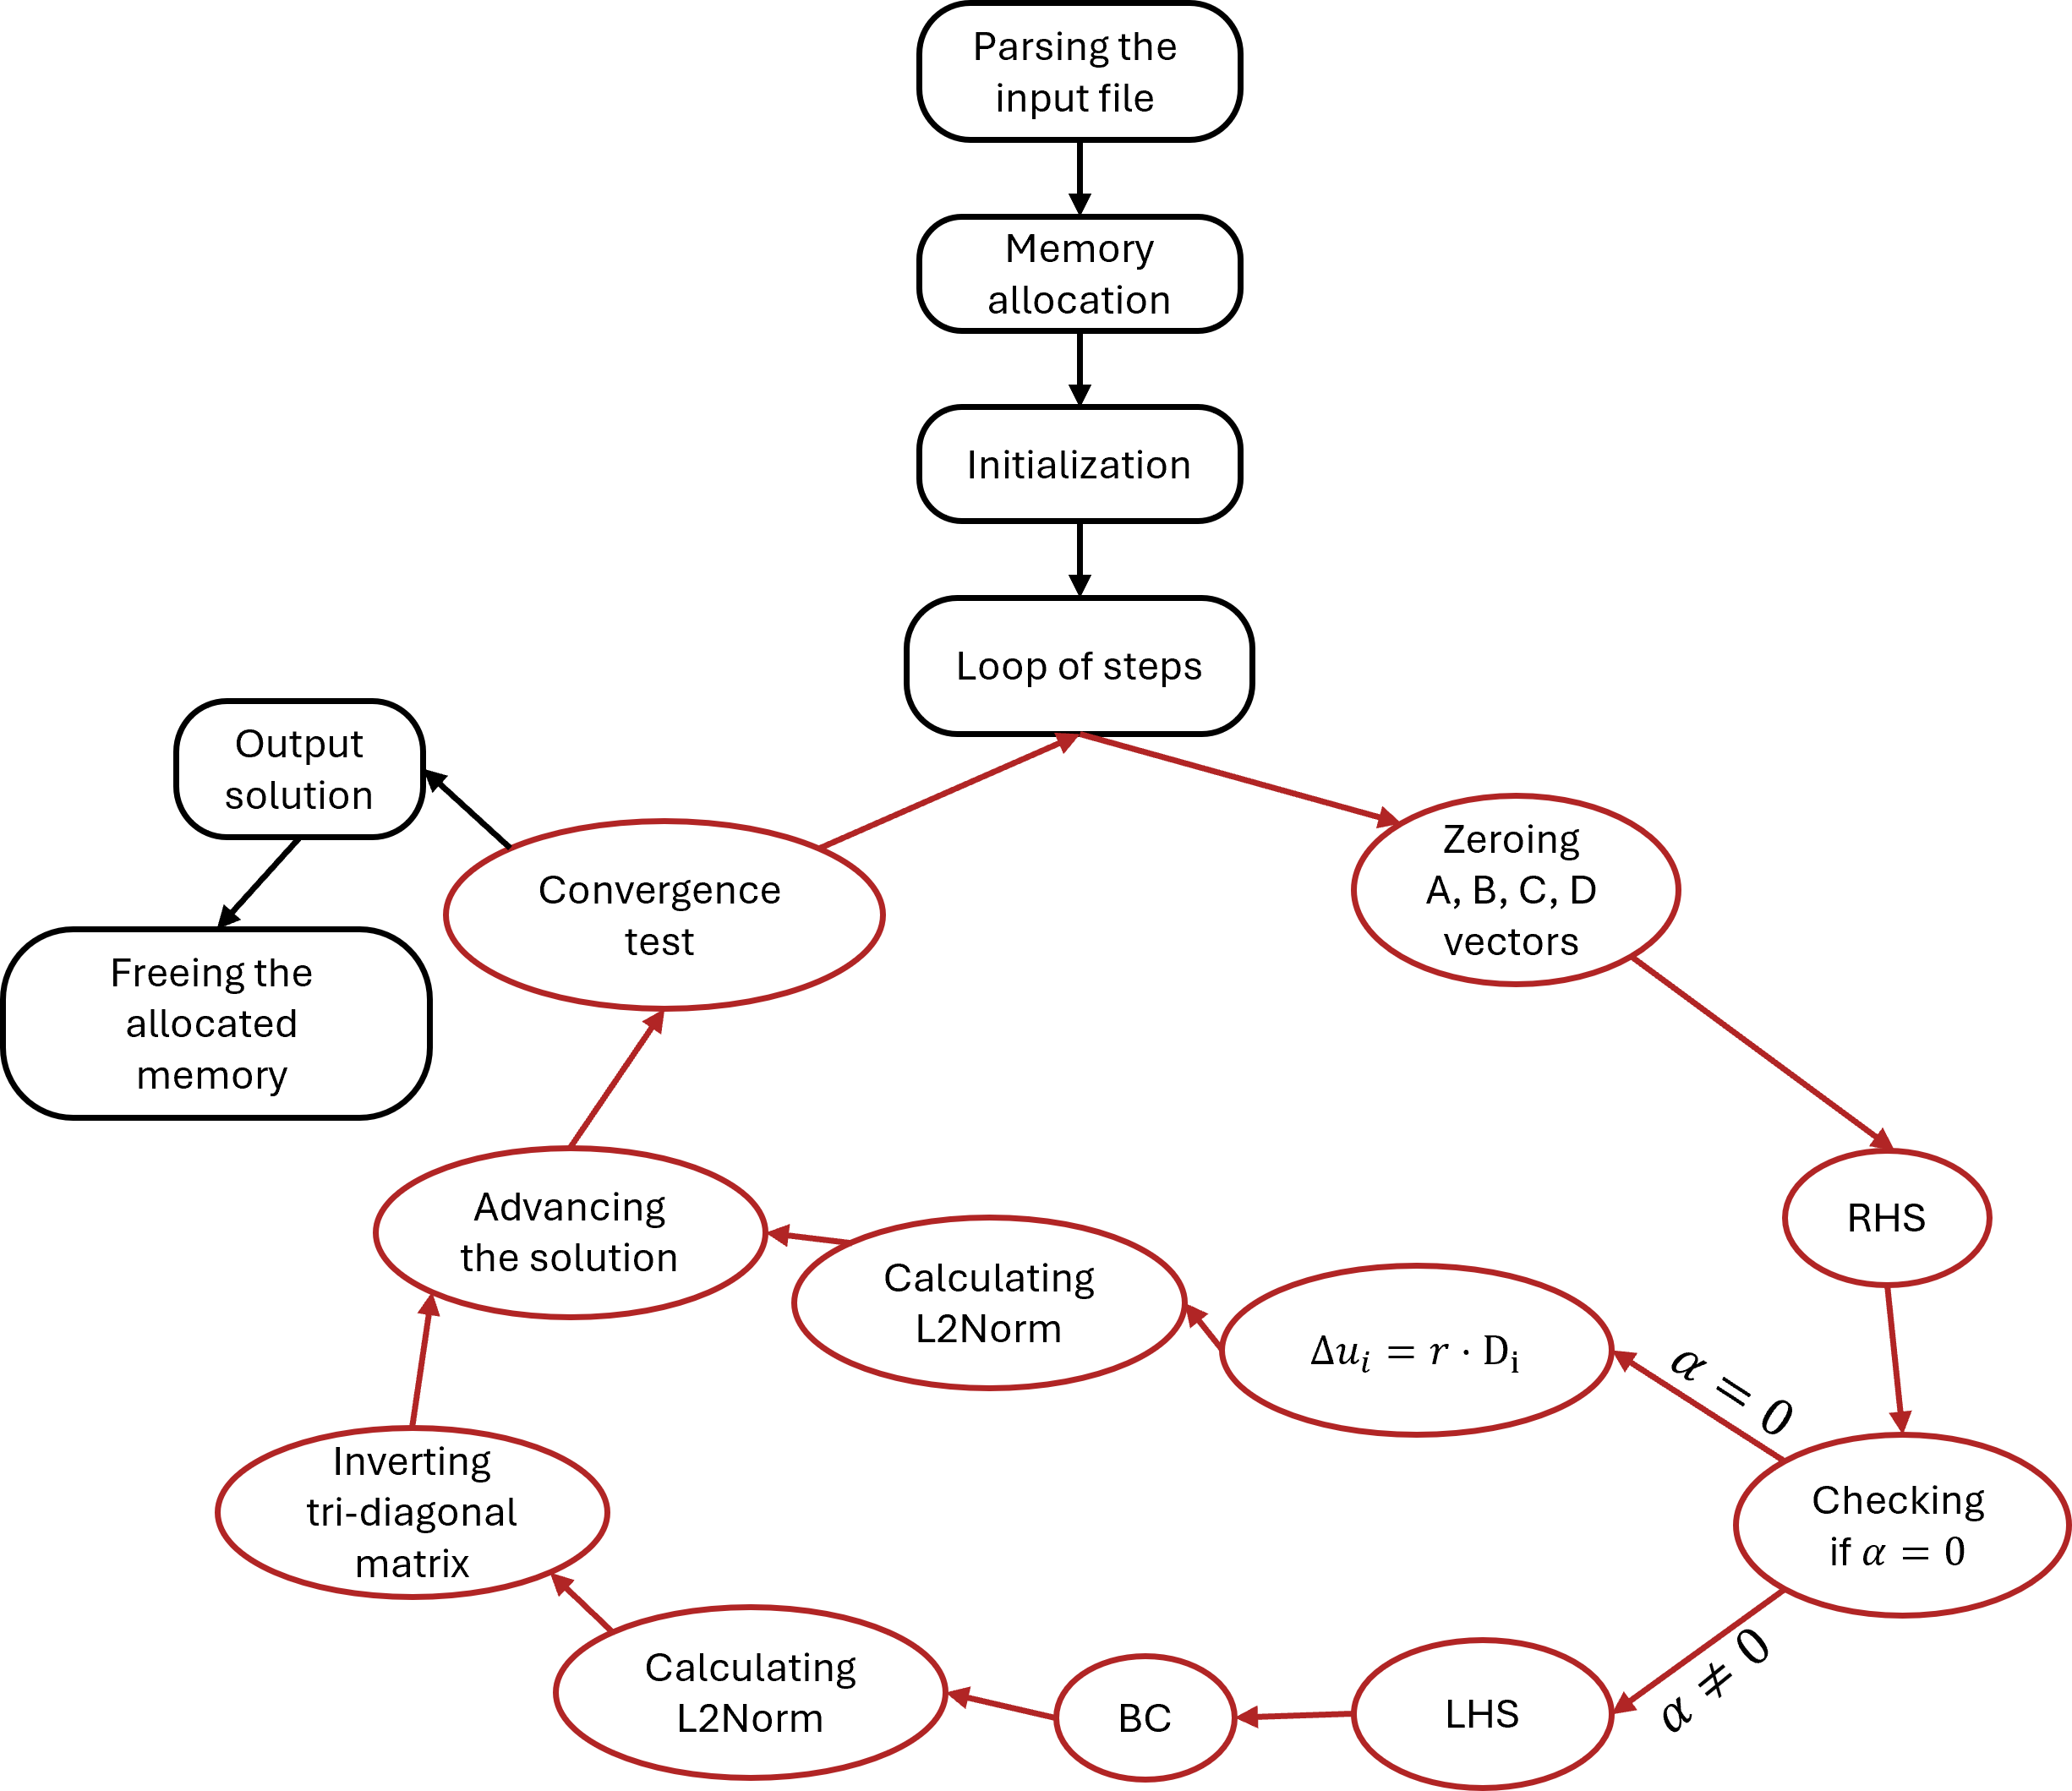
\includegraphics[width=\textwidth]{images/flow chart.png}
    \caption{Flow Chart of the program}
    \label{fig:fl_ch}
\end{figure}
\subsection{The Functions in the Program}
The functions that are included in the program and explanations about them are included in the code itself.

\newpage

\section{Results}
\subsection{$\alpha = 0$ - Explicit Scheme}
From Eq.\ref{eq45} we get the stability limit of $\Delta t$:
\begin{equation}
    \Delta t < \frac{\Delta y^2}{2\mu} = \frac{0.1^2}{2\cdot1} = 5\cdot10^{-3}
    \label{eq:clc_delta_t}
\end{equation}
\begin{figure}[H]
    \centering
    \includegraphics[width=.8\textwidth]{images/grap1.png}
    \caption{Convergence history for $\alpha=0$ for different $\Delta t$}
    \label{fig1}
\end{figure}
\noindent In Figure \ref{fig1} we see that indeed for $\Delta t>5\cdot10^{-3}$ the solution diverges.
Moreover, the number of iterations grows linearly with respect to $\Delta t$.
\begin{figure}[H]
    \centering
    \begin{subfigure}[b]{.49\textwidth}
        \centering
        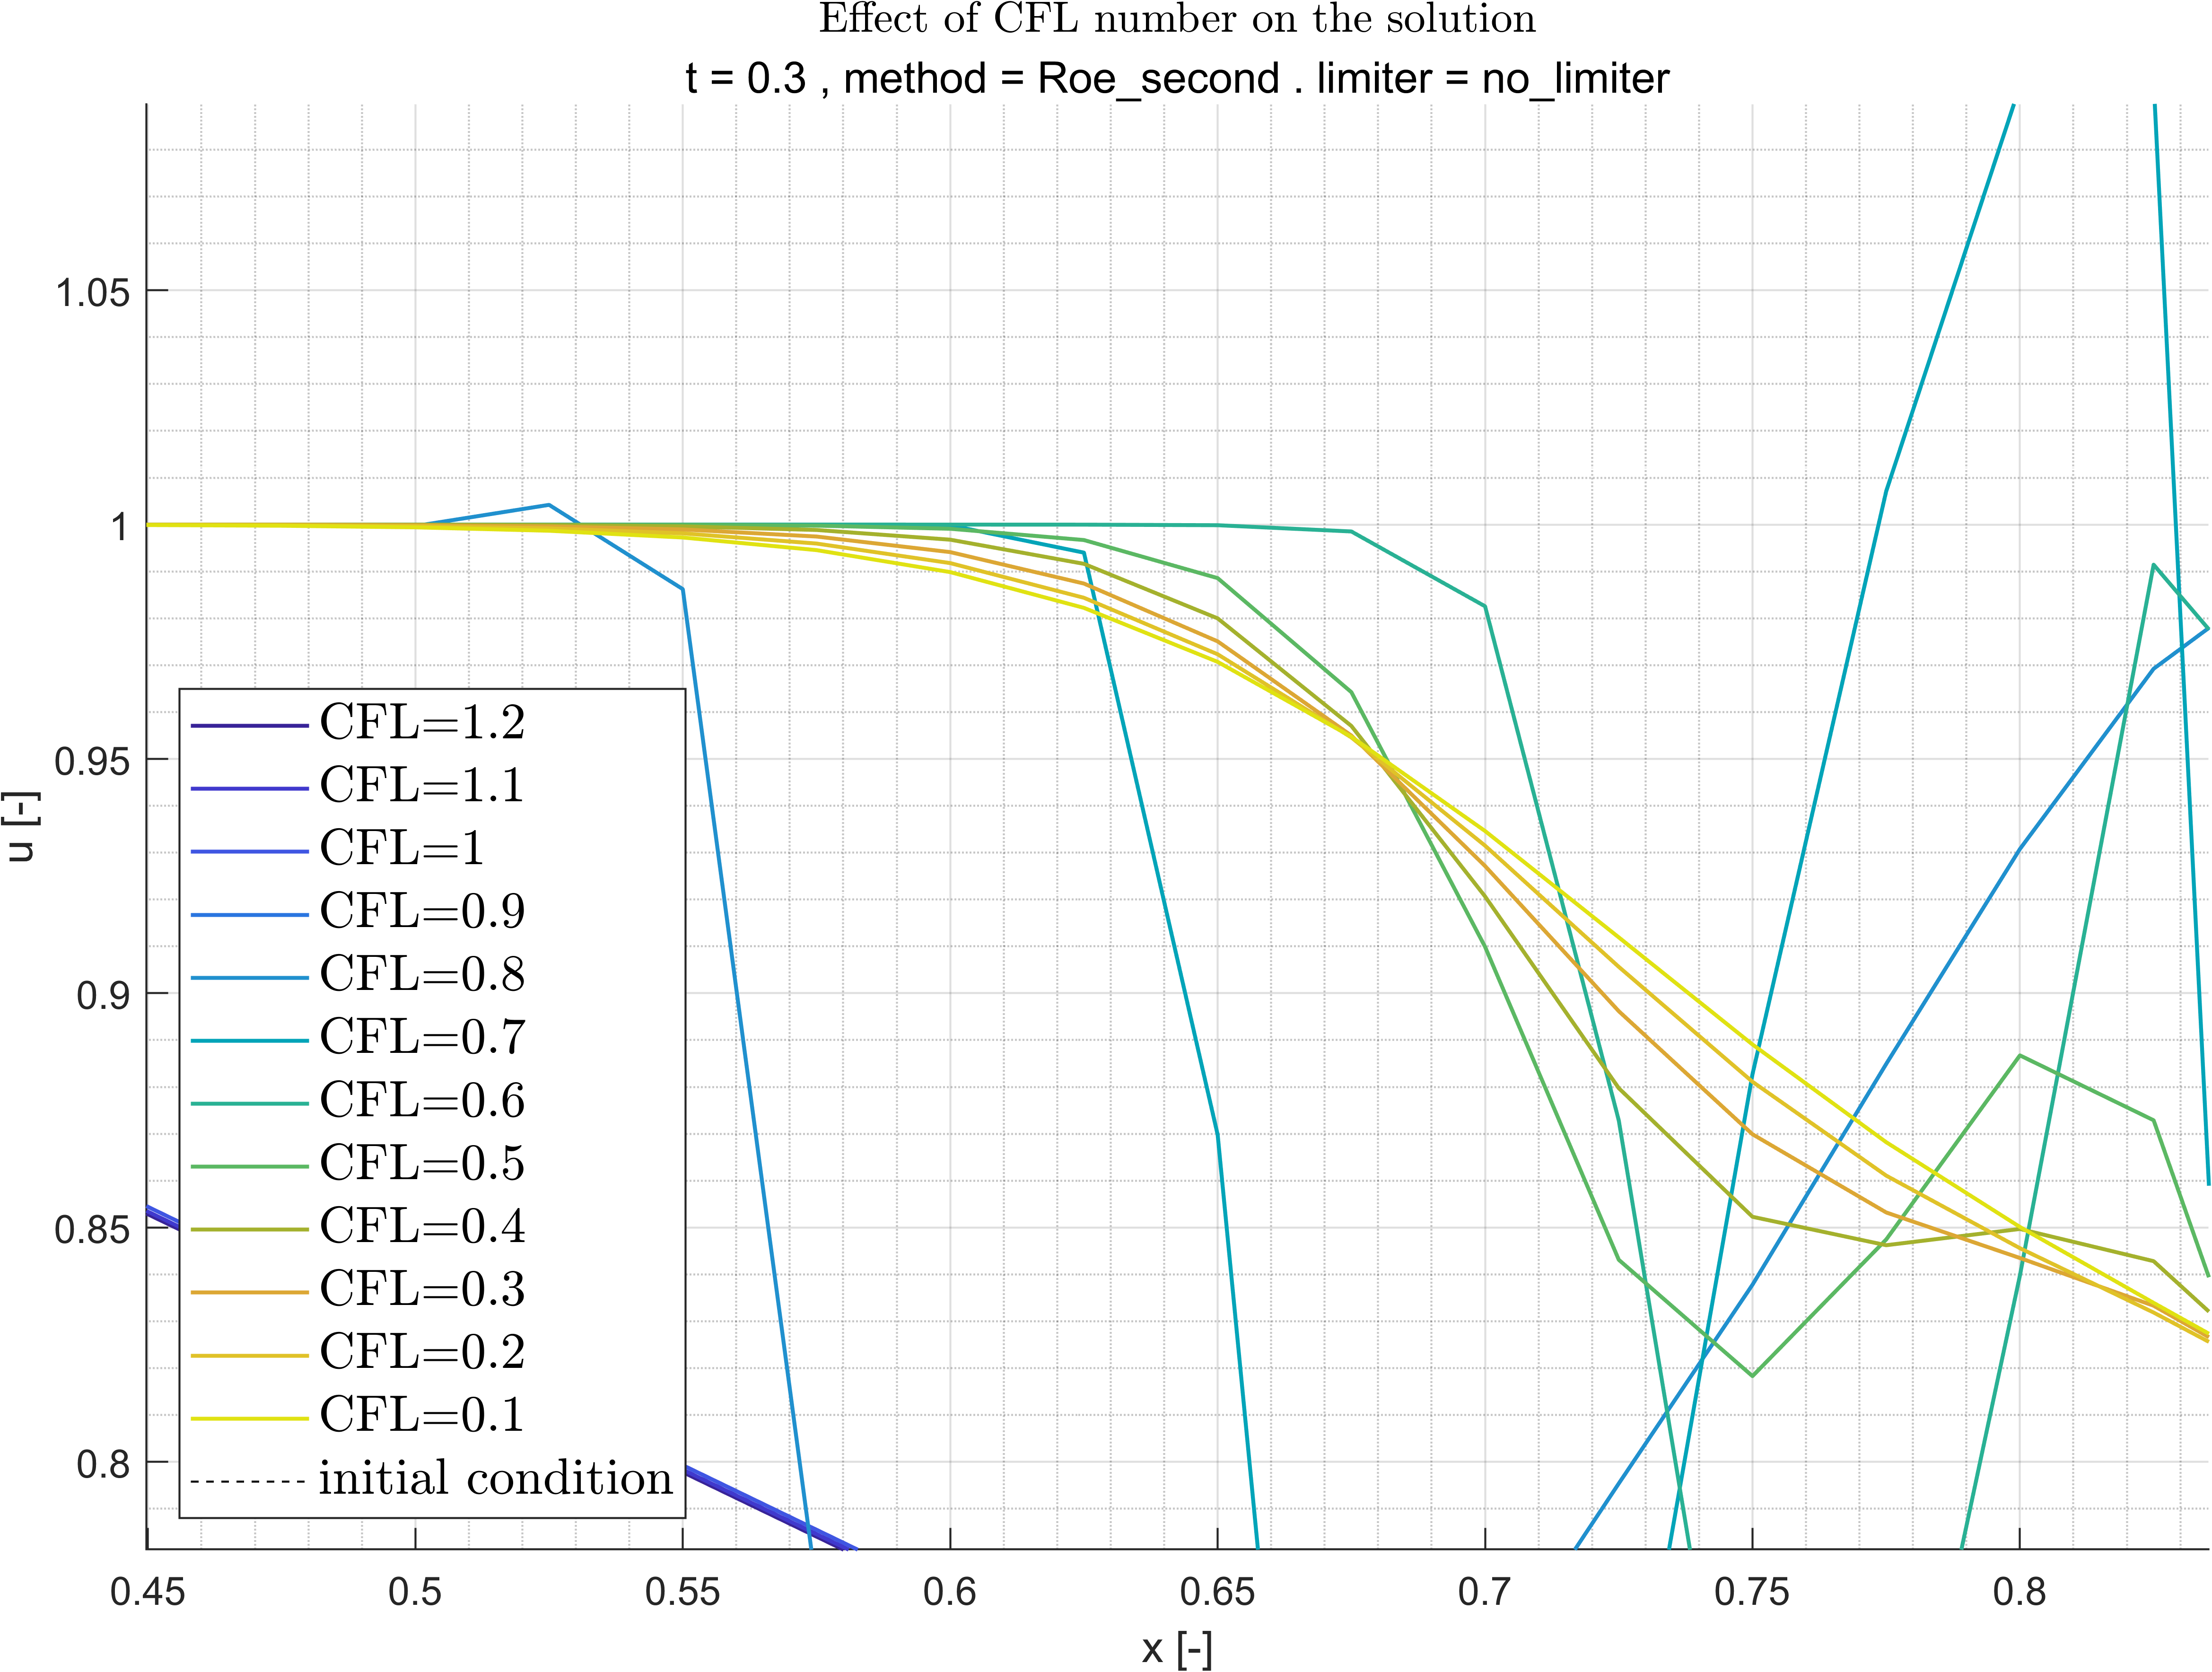
\includegraphics[width=\textwidth]{images/grap2.1.png}
        \caption{Regular view}
        \label{fig2A}
    \end{subfigure}
    \hfill
    \begin{subfigure}[b]{.49\textwidth}
        \centering
        \includegraphics[width=\textwidth]{images/grap2.2.png}
        \caption{Zoomed}
        \label{fig2B}
    \end{subfigure}
    \caption{Effect of $\Delta t$ on solution for $\alpha =0$}
    \label{fig2}
\end{figure}
\noindent In Figure \ref{fig2} we see that when the solution converge, $\Delta t$ has a small effect on the solution. As $\Delta t$ increases, the error increases as well.\\
\noindent The two lines in Figure \ref{fig2A} are the solutions for $\Delta t$ bigger then $5\cdot10^{-3}.$

\newpage
\subsection{$\alpha = \frac{1}{2}$ - Crank-Nicolson Scheme}
From the stability analysis we get that for $\Delta t = \infty$, the scheme is neutrally stable and for every othre $\Delta t$, the scheme converges.
\begin{figure}[H]
    \centering
    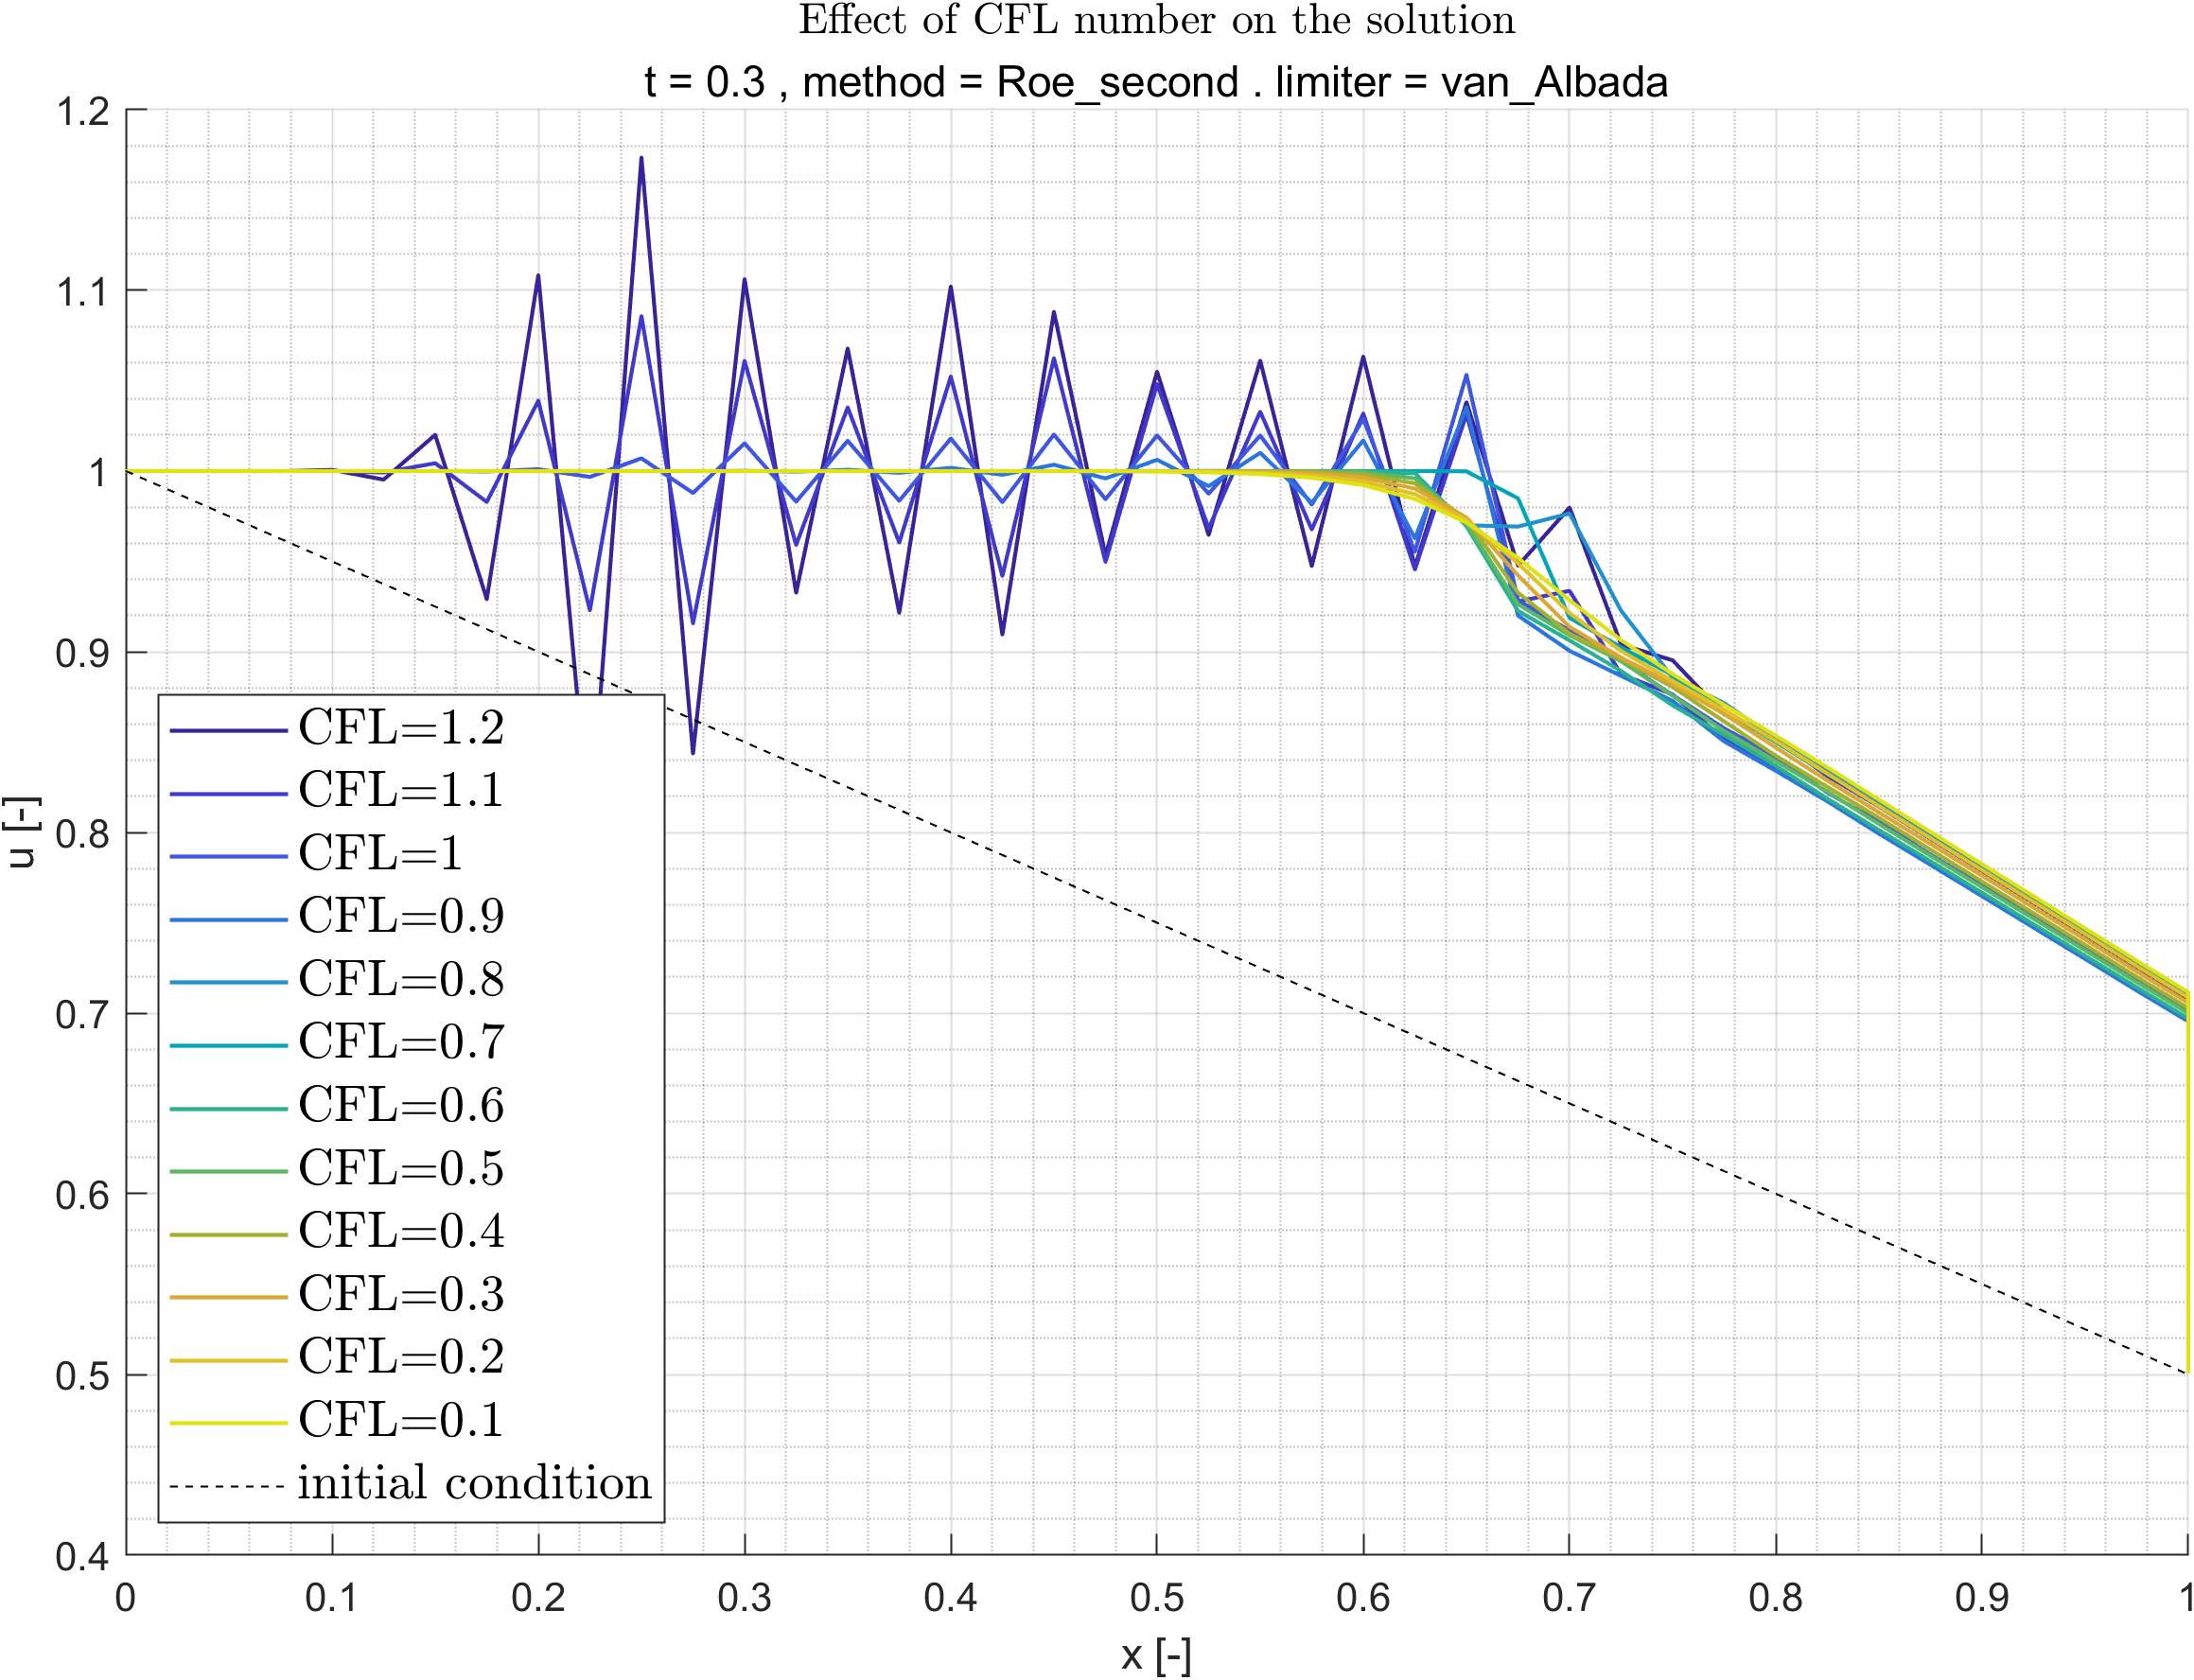
\includegraphics[width=.8\textwidth]{images/grap3.png}
    \caption{Convergence history for $\alpha=0.5$ for different $\Delta t$}
    \label{fig3}
\end{figure}
\noindent In Figure \ref{fig3} that the stability analysis is correct. For $\Delta t = \infty$, the scheme is neutrally stable and for every othre $\Delta t$, the scheme converges. Furthermore, there is an optimal $\Delta t$ for Which the minimal number of iterations is obtained (between $1\cdot10^{-1}$ and $1\cdot10^{-2}$) and the number of iterations is symmetric around that value.
\begin{figure}[H]
    \centering
    \begin{subfigure}[b]{.49\textwidth}
        \centering
        \includegraphics[width=\textwidth]{images/grap5.1.png}
        \caption{Regular view}
        \label{fig4A}
    \end{subfigure}
    \hfill
    \begin{subfigure}[b]{.49\textwidth}
        \centering
        \includegraphics[width=\textwidth]{images/grap5.2.png}
        \caption{Zoomed}
        \label{fig4B}
    \end{subfigure}
    \caption{Effect of $\Delta t$ on solution for $\alpha =0.5$}
    \label{fig4}
\end{figure}
\noindent In Figure \ref{fig2} we see that when the solution converge, $\Delta t$ has a small effect on the solution. As $\Delta t$ increases, the error increases as well.\\
For $\Delta t$ larger then $1\cdot10^{-1}$ that still converges, the numerical solution is identical to the analytical one.
\begin{figure}[H]
    \centering
    \begin{subfigure}[b]{.49\textwidth}
        \centering
        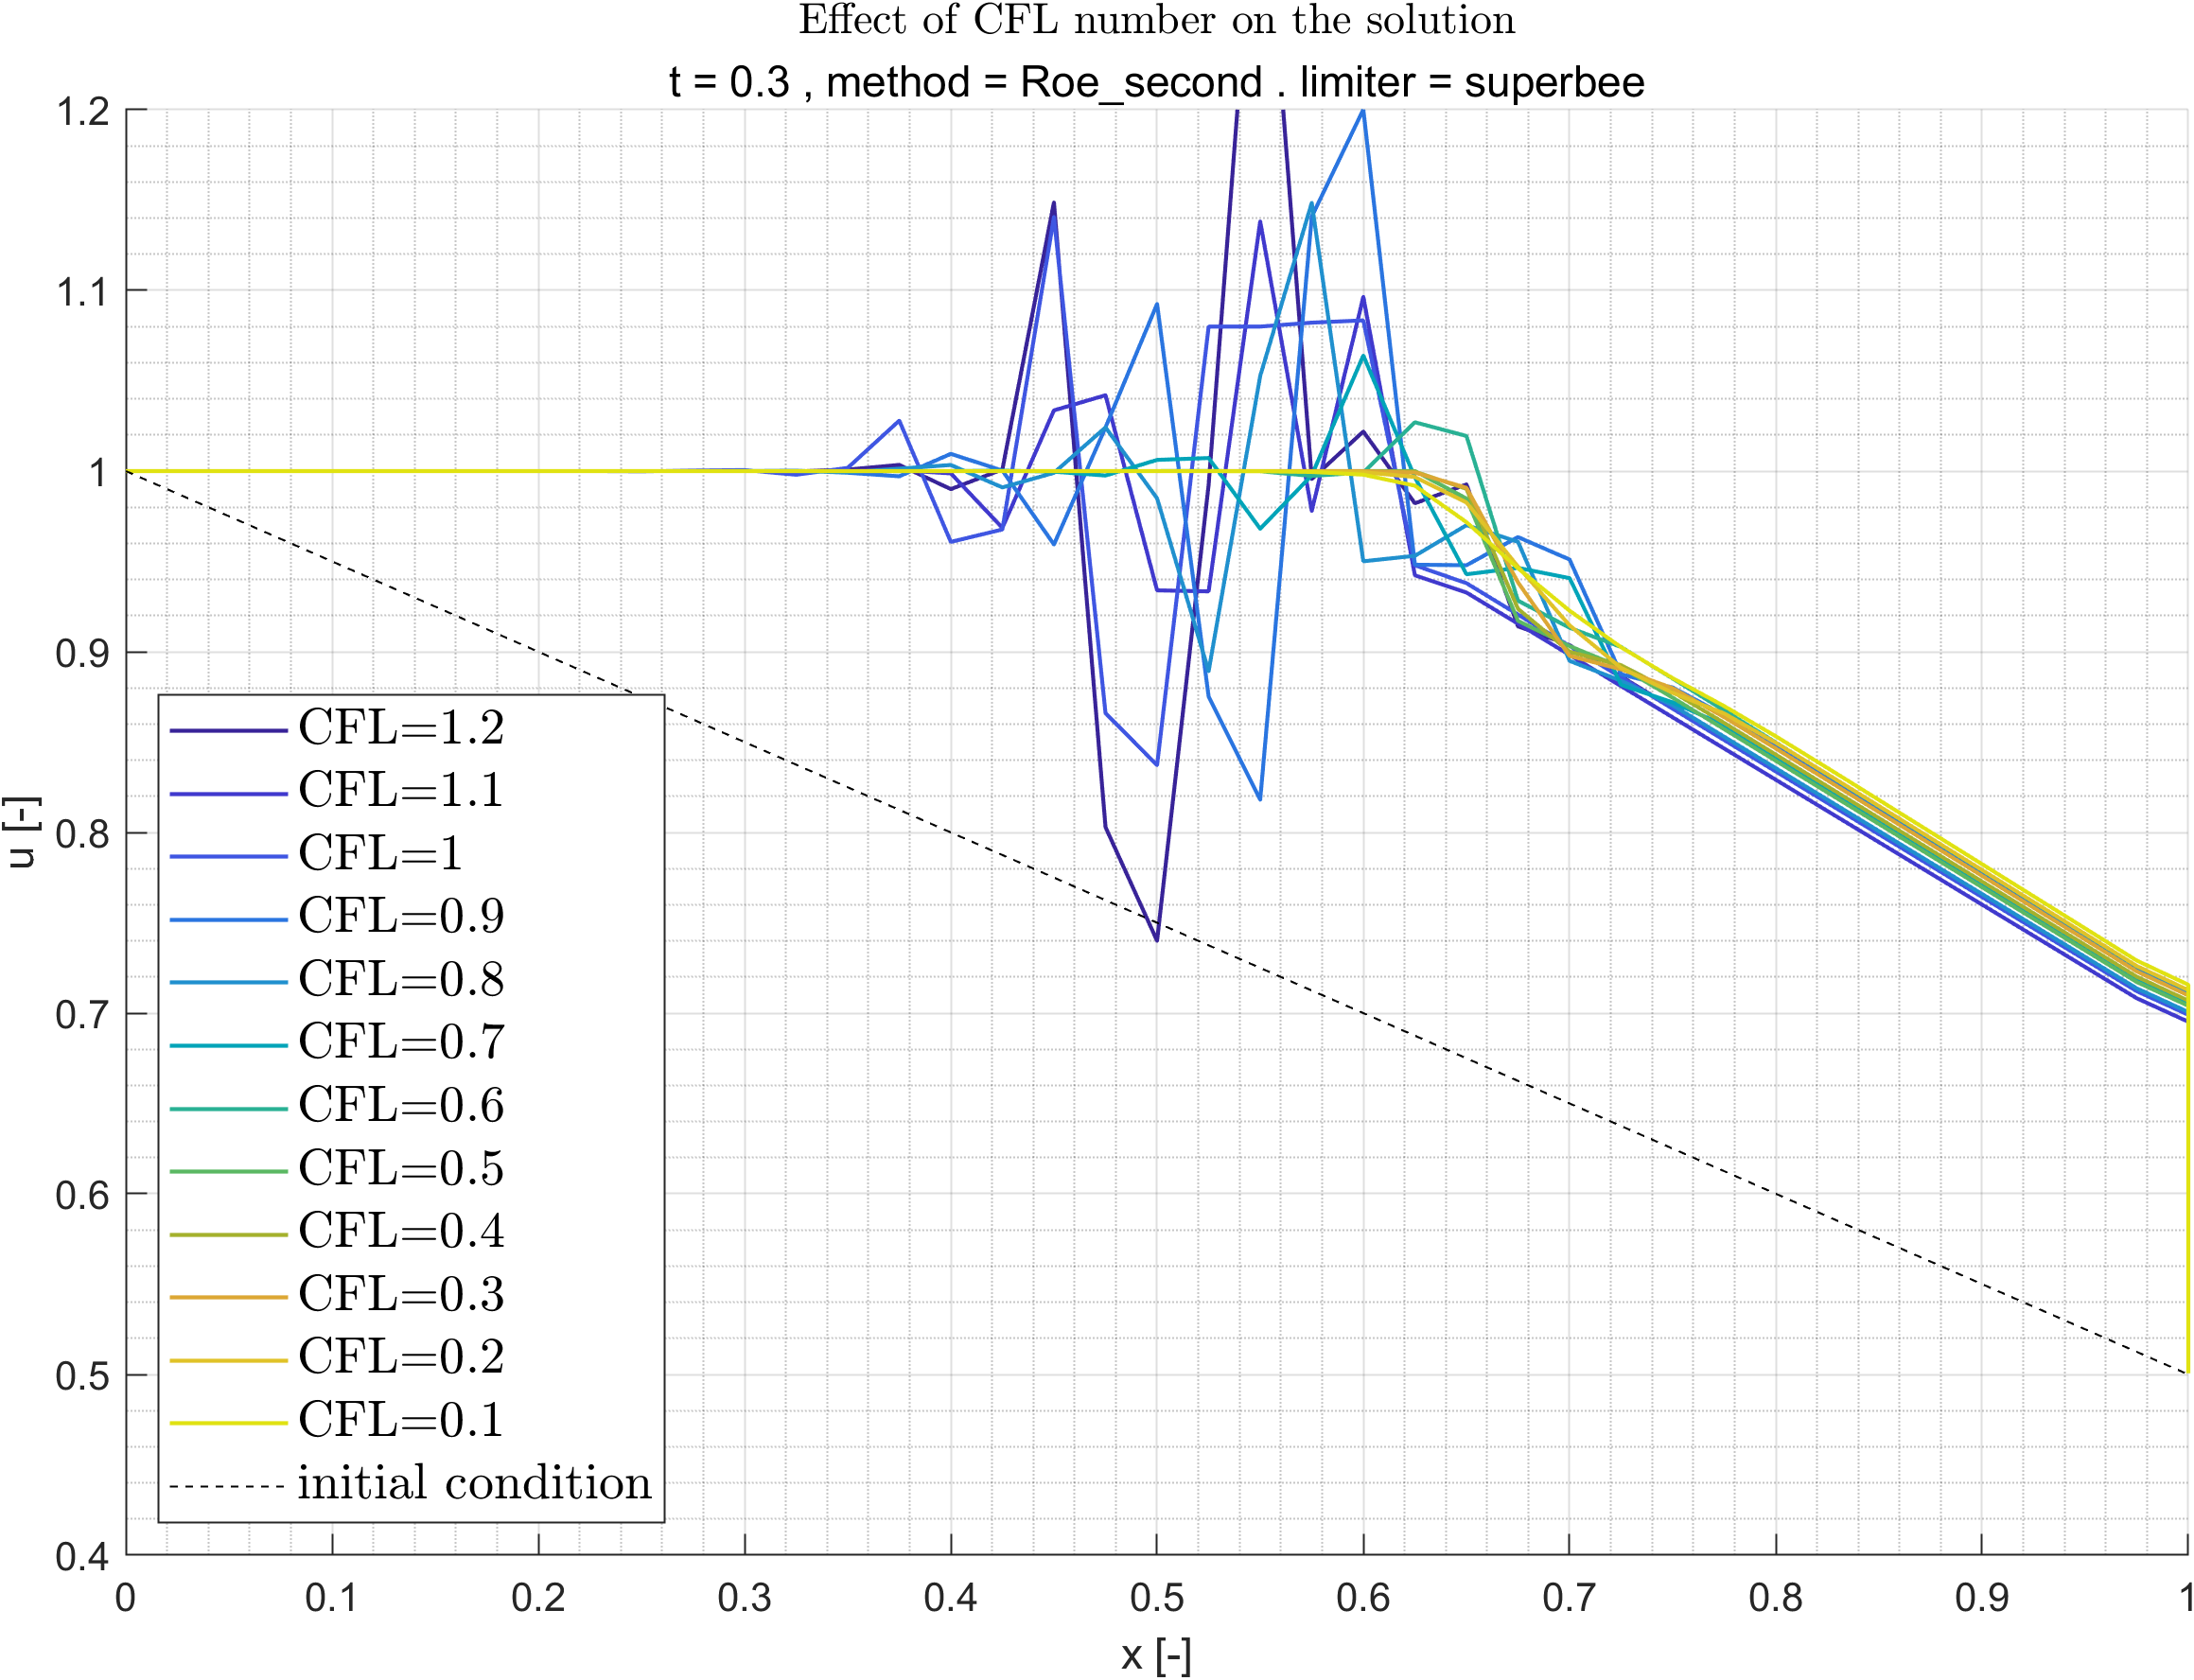
\includegraphics[width=\textwidth]{images/grap4.png}
        \caption{$\Delta t = 10$}
        \label{fig5A}
    \end{subfigure}
    \hfill
    \begin{subfigure}[b]{.49\textwidth}
        \centering
        \includegraphics[width=\textwidth]{images/grap6.png}
        \caption{$\Delta t = \infty$}
        \label{fig5B}
    \end{subfigure}
    \caption{Oscillation of solution for Crank-Nicolson}
    \label{fig5}
\end{figure}
\noindent In Figure \ref{fig5A} we can see the oscillation of the solution that occur when $ 10^{-2} < \Delta t < \infty$. The even iterations are above the analytical solution and the odd iterations are below.\\
Figure \ref{fig5B} showed the perferct oscillation that happens when $\Delta t=\infty$ in the Crank-Nicolson scheme and the meaning of \emph{neutrally stable}. The distance of the even iterations from the analytical solution is exactly the distance of the odd iterations from the analytical solution.

\subsection{$\alpha = 1$ - Implicit Scheme}
For the implicit scheme, the stability analysis states that the scheme is stable for every $\Delta t$.
\begin{figure}[H]
    \centering
    \includegraphics[width=.8\textwidth]{images/grap7.png}
    \caption{Convergence history for $\alpha=1$ for different $\Delta t$}
    \label{fig6}
\end{figure}
\noindent Figure \ref{fig6} validates the Stability analysis and shows clearly that for every $\Delta t$ the solution converges. Moreover, for $\Delta t>1\cdot10^{10}$, the solution converges immediately.
\begin{figure}[H]
    \centering
    \begin{subfigure}[b]{.49\textwidth}
        \centering
        \includegraphics[width=\textwidth]{images/grap8.1.png}
        \caption{Regular view}
        \label{fig7A}
    \end{subfigure}
    \hfill
    \begin{subfigure}[b]{.49\textwidth}
        \centering
        \includegraphics[width=\textwidth]{images/grap8.2.png}
        \caption{Zoomed}
        \label{fig7B}
    \end{subfigure}
    \caption{Effect of $\Delta t$ on solution for $\alpha =1$}
    \label{fig7}
\end{figure}
\noindent Unlike every other scheme, the implicit solution converges for every $\Delta t$ as seen clearly in Figure \ref{fig7A}. From Figure \ref{fig7B} we can see that the smaller $\Delta t$ is, the larger the error and for $\Delta t$ bigger then $1$, the solution is exactly the analytical one. 


\section{Conclusions}
\subsection{$\alpha = 0$ - Explicit Scheme}
\begin{itemize}
    \item As seen in Figure \ref{fig1}, the $\Delta t$ derived from Eq.\ref{eq:clc_delta_t} is indeed the stability limit for the \emph{Explicit Scheme}.
    \item The number of iterations increases linearly with respect to $\Delta t$ for $\Delta t$ smaller then the limit in Eq.\ref{eq45}.
    \item The deviation from the analytical solution increases as $\Delta t$ decreases.
\end{itemize}
\subsection{$\alpha = \frac{1}{2}$ - Crank-Nicolson Scheme}
\begin{itemize}
    \item The oscillation around the analytical solution for $\Delta t= \infty$ happens because:
    \begin{equation}
         - \underbrace{\alpha}_\frac{1}{2}\delta_{yy}\left(\Delta u^n_i\right) = \delta_{yy}\left(u^n_i\right)
    \end{equation}
    Which means that the correction is exactly twice the distance to the analytical solution.
    \item In Figure \ref{fig3} we see that indeed for every finite $\Delta t$ the solution converges.
    \item Unlike the implicit scheme, for $\Delta t > 1\cdot10^{-1}$ the number of iterations until convergence increases.
\end{itemize}
\subsection{$\alpha = 1$ - Implicit Scheme}
\begin{itemize}
    \item Figure \ref{fig6} verifies that, as the stability analysis states, the \emph{implicit scheme} is stable for every $\Delta t$.
    \item From Figure \ref{fig6} we can determt that the number of iterations increases as $\Delta t$ increases and when $\Delta t > 10^{10}$ the solution converges immediately.
    \item In Figure \ref{fig7B} we see that the error increases as $\Delta t$ decreases.
\end{itemize}

\end{document}
